%!TEX root=../master.tex

\newcommand{\policy}[2]{\ensuremath{#1\!:\;#2}}

\section{Decentralized Label Model}
The Decentralized Label Model (DLM) is a modern information flow control model devised in 1999.\cite{myers1999mostly}
As the name suggests it revolves around labels (similar to previous security models), however, DLM is decentralized.
This means that it can be applied to systems with no trusted third party, or even any trust throughout the system.
By attaching security labels to objects in code it can be controlled how information should be shared throughout the code and at code-endpoints (input/output to/from other programs).
It is possible to do both static and run-time checking of labels.
The final major point of DLM is that it is formalized and even though no implementation is supplied, it should be applicable to other existing programming languages.

\newcommand{\xvalue}{value}
\newcommand{\xvalues}{values}

\subsection{Labels}
A \xvalue{} is associated with a label.
The label is a set of privacy policies.
When the \xvalue{} flows through the system, all the policies need to be obeyed.
This means that the effective set of \principals{} able to read the \xvalue{} is the intersection of all policies in a label.

A privacy policy is represented as an owner of some \xvalue{} and a set of readers.
The syntax is: $\policy{\text{<\emph{owner}>}}{\text{<\emph{reader}>}}$.
The owner is the \principal{} who owns the \xvalue{} that was used for constructing the \xvalue{}.
The readers are the \principals{} allowed by the owner.
The owner is implicitly allowed to read his own data.
If we want a \principal{} $p$ that should not allow any other readers we provide an empty reader list: $\policy{p}{}$.

If we have policy $K$ and label $L$, we have following notation:
\begin{itemize}
\item $K \in L$, policy $K$ is a part of label $L$
\item $\textbf{o}(K)$, the owner of policy $K$
\item $\textbf{r}(K)$, the set of readers of policy $K$
\end{itemize}

Labeled \xvalues{} are only released by the consensus of all the owners and can only be read by the readers.
If one or several privacy policies are added to a label it restricts the access to the \xvalue{}.
A label with no policies  means that all readers are allowed.

If a \principal{} is not among the owners of a label, it is the same as if it was added as a privacy policy with all posible readers, implicitly indicating that this owner has no preference of who reads the \xvalue{}.

\begin{example}{Redundant owner}
In a system with owners $o_1, o_2, o_3$ and readers $r_1, r_2, r_3$, the following labels are defined:
$$L_1 = \{\policy{o_1}{r_1,r_2};\; \policy{o_2}{r_2, r_3}\}$$
$$L_2 = \{\policy{o_1}{r_1,r_2};\; \policy{o_2}{r_2, r_3};\; \policy{o_3}{r_1, r_2, r_3}\}$$
Since the policy of $o_3$ is to allow everyone to read it introduces no restriction to the label.
Therefore we say that the effective reader set of the two labels are equal.
\end{example}

A label can contain several privacy policies for the same \principal{}.
These are enforced just as other policies.

\subsection{Rules}
This section contains the rules that need to be followed when manipulating labels to avoid information leakage.
The modification of labels is what makes it possible to define how data flows through a system.

\paragraph{Label join}
When deriving a \xvalue{} from two \xvalues{}, the label of the derived \xvalue{} must reflect its sources, so it has to be at least as restrictive.
The relation $\sqsubseteq$ determines that a label is \textit{at least as restrictive}.
\begin{definition}
  For two labels $L_1$ and $L_2$, if we have $L_1 \sqsubseteq L_2$, $L_1$ is at least as restrictive as $L_2$.
  Then, in order to keep the restrictiveness of a combination of two labels, the resulting label for a derived \xvalue{} is the union of the two source labels.
  This gives us the following join rule:
  \begin{center}
    $L_1 \sqcup L_2 = L_1 \cup L_2$
  \end{center}
\end{definition}

The join rule will ensure that any joining of values will also result in a joining of labels, so that any combination of rules will be upheld.

\paragraph{Relabeling by declassification}
The owners of the labels control their data, but sometimes policies are overly restrictive and one wants to relax them.
This can be used to sanitize \xvalues{} whose security policies, in respect to one ore more owners, have changed throughout the run of a program.
This works in opposition to restricting rules, which is used to ensure information is not leaked, whereas this is enabling intended leaking (of sanitized information).

The authority is a set of \principals{} which is the authority of the process of declassification.
If a process has the authority of a \principal{}, the actions of the process are permitted.
This means that if a \principal{} is in the authority set this can be declassified.

\begin{definition}
  A label $L_1$ can be relabeled to $L_2$ if $L_1 \sqsubseteq L_2 \sqcup L_A$ where $L_A$ is the authority.
  The authority is a label $L_A$ of the form $\{p: \ \}$ for every \principal{} in the current authority.
  $L_1$ can be relabelled to $L_2$ if $L_1 \sqsubseteq L_2 \sqcup L_A$ is true.
  \begin{center}
    \[\frac{L_1 \sqsubseteq L_2 \sqcup L_A}{L_1 \text{ may be declassified to } L_2}\]    
  \end{center}
\end{definition}
\stefan{Jeg synes desclassification er rodet. Hvor kommer authority fra, og hvordan indikerer man det? Definition 2.9 ser ud til at sige det samme flere gange (noget med  $L_1 \sqsubseteq L_2 \sqcup L_A$, men jeg er ikke sikker på om det er forskellige pointer)}

\paragraph{Relabeling by Restriction}
When a \xvalue{} is read from a variable it has the same label as the variable.
When a \xvalue{} is stored in a variable the label of the \xvalue{} is forgotten.
\begin{example}{Assignment}
  Given $a = 4$, and we want to assign the value of another variable, $b$, to $a$.
  First we read the \xvalue{} from $a$, this means the \xvalue{} of $a$, $4$, has the same label as $a$.
  Now we assign the copied \xvalue{}, $4$, to $b$, this means the \xvalue{} gets the label of the variable $b$, replacing its own label.
  This means that the label that the \xvalue{} got from $a$ is forgotten.
\end{example}
This example shows the process of what we call relabeling, and more specifically this kind of relabeling is called restriction.
\stefan{ikke forstået. Hvad er resultatet? Hvad er a bagefter? Hvor bliver 4 af? (Væk i assume, men 4's label bliver ændret undervejs)}

To avoid leakage the label of the variable must be at least as restrictive.
For instance if we have two labels, $L_1$ and $L_2$, $L_1 \sqsubseteq L_2$ means that $L_2$ is more restricted than $L_1$.

\begin{definition}
  A restriction is when the new label guarantees to enforce all of the policies from the old label.
  If we have policy $J$ in $L_1$ it is guranteed by another policy $K$ if they have the same owner and $r(K)$ is a subset of $r(J)$.
  \begin{center}
    \[\frac{\forall (J \ \in \ L_1) \exists (K \ \in \ L_2)(o(K) = o(J) \ \wedge \ r(K) \subseteq r(J))}{L_1 \sqsubseteq L_2}\]    
  \end{center}
\end{definition}
\stefan{burde det ikke introduceres tidligere? $\sqsubseteq$ bliver brugt mange gange før }

\subsection{Acts-for relation}
A \principal{} in DLM can represent a user in the system, a group of users or roles.
As labels on slots are immutable, in order to have more dynamic security policies we have that \principals{} are able to \textit{act for} other \principals{}.
This means that a given \principal{} in effect has every right that the \principal{} that it acts for has.

This is also called a \principal{} hierarchy.
Formally we use the $\succeq$-operator when representing acts for.\footnote{$\succeq$ is reflexive and transitive and not anti-symmetric.}
For instance $x \succeq y$ means $x$ acts for $y$.
A \principal{} hierarchy $P$ is a set of ordered pairs of \principals{}.
So if we have $P \vdash x \succeq y$ it means that $(x,y) \in P$.

Some examples:
\begin{example}{Acts-for relation}
  Given the acts-for relation and \principals{} $Amy$ and $Bob$, $Amy \succeq Bob$ means that Amy \textit{acts for} Bob.
  Any security policies that apply to Bob will in effect also apply to Amy.
\end{example}
\begin{example}{Acts-for relation groups}
  Groups or roles are no different than any other principal -- given a new \principal{} $Admin$ we can have that $Amy \succeq Admin$, signifying that Amy is an administrator and therefore can act for on behalf of the administrator group. 
\end{example}
\subsection{Channels}
The model contains two types of channels, input and an output channels.
Information can be leaked through these channels, therefore they have a label associated to them.
When a \xvalue{} enters the system through an input channel, the \xvalue{} gets the label of the input channel.
If a \xvalue{} is written to an output channel it can only be done if the label of the output channel is at least as restrictive as the label of the \xvalue{}.

\subsection{Smart Meter System Example}\label{dlm-example}
In order to give some idea about how the DLM could be used, we provide an example of a smart meter system while displaying the different principals (actors) and labelled objects.
This is similar to the provided motivating examples presented in \citet{myers1997decentralized}.

\begin{figure}[h]
\centering
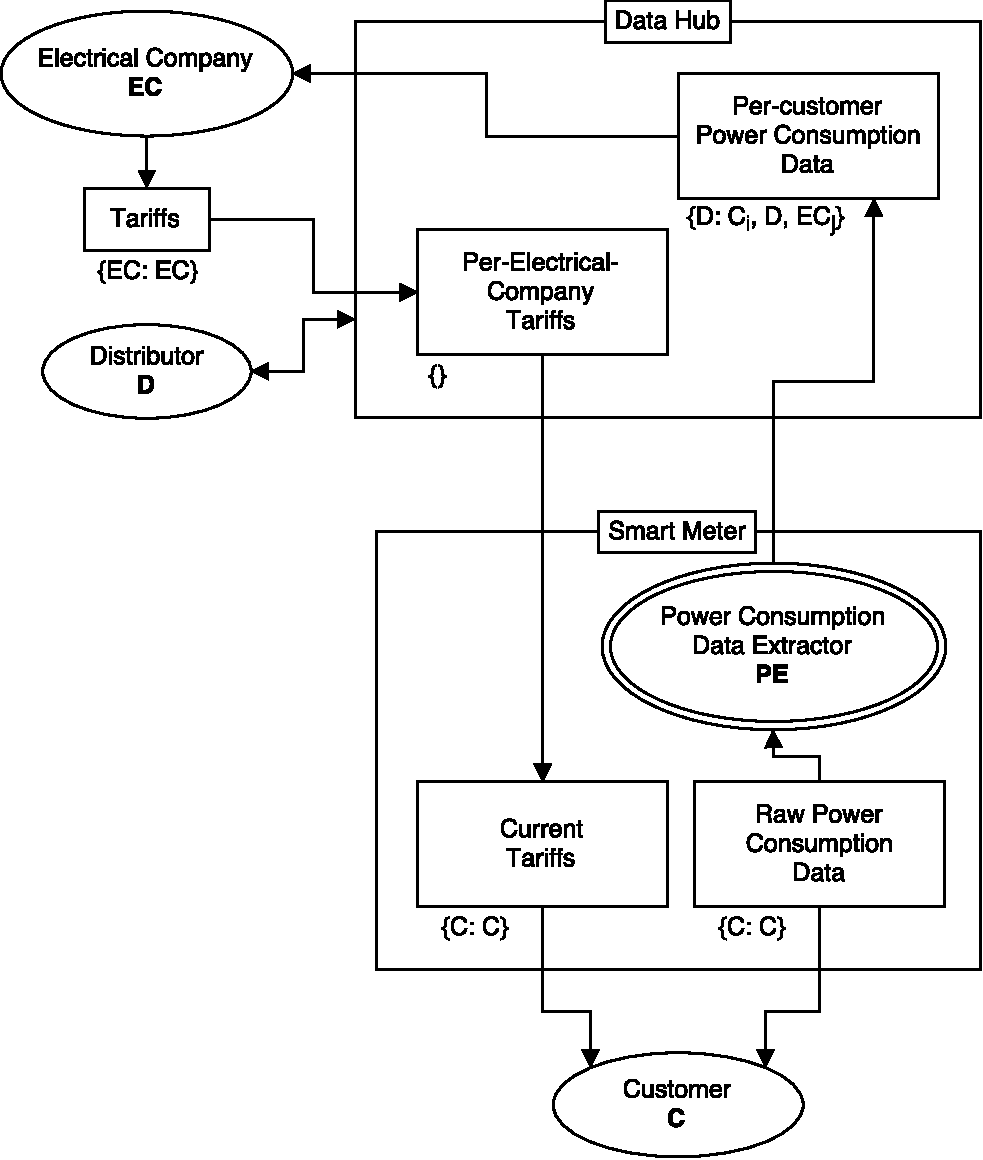
\includegraphics[width=\textwidth]{figures/dlm_sm_example.pdf}
\caption{Abstract smart meter system with DLM principals and labelled objects}
\label{dlm:sm_example}
\end{figure}

In \cref{dlm:sm_example} can be seen the abstract smart meter system, with principals (ovals), labelled objects (rectangles), and trusted agent (double oval).
\stefan{Hvad er en trusted agent?}
Arrows display how information flows.
There are two overall components to this system: the Data Hub and the Smart Meter.
The rectangles used for these components signify only a grouping of objects.

Initially, consumers own the data contained in their smart meter, most importantly the raw consumption data.
$PE$ extracts the consumption data and transforms it into a granularity that does not reveal information about the consumer.
In order for the distributor and electrical company to carry out their tasks, balancing the electrical grid and correctly billing, they have access to the transformed power consumption data.
Inside the Data Hub, the distributor receives ownership of all consumption data\footnote{This is actually unclear, but not important to discuss at this point}, but for the power consumption data for each individual consumer $C_i$ the only allowed additional reader is the current electrical company of $C_i$: $EC_j$.
In case $C_i$ changes to a new electrical company $EC_k$, the read access must be removed from $EC_i$ and given to $EC_k$.

The different electrical companies will also provide their current tariffs to the data hub, so that they can be sent to the smart meters and for anyone to see the pricing of available electrical companies in case they want to switch supplier.
The label is empty so that anyone can read the tariffs.
